\chapter{Einleitung}

In einer vernetzten Welt senden Geräte Daten über ihren Zustand oder den ihrer Umgebung. Diese Technologie wird für eine Fahrradfahrerin bzw. einen Fahrradfahrer nutzbar gemacht. Das Handy soll die aktuelle Geschwindigkeit, die Höhe über Meer, die Temperatur und die Luftfeuchtigkeit während der Fahrt empfangen.

Diese Idee ist nicht neu. Erhältlich sind batteriebetriebene Modelle (siehe \ref{ausgang}), die Daten auf einem Display anzeigen. Das Neue an dieser Arbeit ist, dass die Energie aus der Fahrradumdrehung geerntet (engl. to harvest) wird und dass die Benutzerin bzw. der Benutzer sein eigenes Handy für das Anzeigen der Daten nutzen kann.


\section{Ausgangslage}
\label{ausgang}

Als Inspiration für den Prototypen dienten zwei batteriebetriebene Modelle der Hersteller Sigma Sport (\cite{SigmaSport}) und Polar (\cite{PolarElectro}). Sigma Sport bietet Geräte mit eigenem Display und  Sensoren an. Auf dem Display erscheinen neben der Geschwindigkeit die Daten der Sensoren, die GPS-Ortung und der aktuelle Ladestand der Batterie. Der Hersteller Polar stellt ein Gerät her, welches die Fahrt über GPS aufzeichnet und wichtige Informationen zur Trainingsverbesserung liefert. Jedoch wird ein (verdrahtetes) Display gebraucht.

Ein weiterer, interessanter Hersteller ist Reelight  (\cite{Reelight}). Reelight gewinnt über Wirbelströme Energie und schafft es, bei seinem Produkt City Supreme genügend Energie für eine LED-Lampe zu erzeugen. Da auf der Webseite keine Dokumentation des Funktionsprinzips erhältlich ist, ergaben eigene Untersuchungen, dass sich im Innern der Lampe ``etwas'' bewegt. Es steht zu Vermutung, dass dies ein Magnet, der so gelagert ist, dass er sich drehen kann. Der an der Felge vorbeiziehende Magnet erzeugt einen Wirbelstrom in der Felge. Der Wirbelstrom wirkt auf den Magneten im Licht. Der Magnet im Licht beginnt sich zu drehen. Befindet sich neben dem sich drehenden Magneten eine Spule, so wird genügend Spannung für das Betreiben einer LED induziert. Diese Harvesting-Methode könnte interessant für eine zukünftige Arbeit sein. Der Nachteil dieser Methode ist, dass das Erzeugen eines Wirbelstroms sich auf den Felgen bremsend auswirkt.  Bei dieser Bachelorarbeit ist die Harvesting-Methode bereits vorgegeben, da sie auf der nachfolgend genannten Projektarbeit basiert (\cite{PA_bicycle}).

Als Grundlage dient der Aufbau aus der Machbarkeitsstudie ``Bicycle computer and sensoric powered with harvested energy'' (\cite{PA_bicycle}). In dieser Projektarbeit wird der Beweis erbracht, dass durch Bewegungsinduktion genug Energie erzeugt werden kann, um die Geschwindigkeit des Fahrrads per Bluetooth Low Energy zu übermitteln. Der Aufbau funktioniert nach vorangehendem Laden der Kondensatoren zuverlässig bei 20 km/h. Das Ziel dieser Arbeit besteht aus einer verbesserten Energiegewinnung aus der Radumdrehung, einem besserem Verbrauchsmanagement bei der Datenverarbeitung durch einen Microkontroller und einer ansprechenden Applikation. Konkret soll ein attraktives Produkt ohne Aufladen der Kondensatoren für eine Geschwindigkeit von 10 km/h entstehen. Dieser Fahrrad-Computer-Prototyp wird in dieser Arbeit kurz Bicycle Computer genannt.



\section{Definition der Aufgabenstellung}\label{Aufgabenstellung} 

Durch die offizielle Ausschreibung der Bachelorarbeit an der ZHAW ist der Inhalt der Bachelorarbeit vorgegeben (siehe Anhang \ref{Ausschreibung}). Das Ziel der Arbeit ist es, aus dem Aufbau einer Machbarkeitsstudie einen Prototypen eines batterielosen Fahrrad-Computers zu entwickeln. Zusammen mit den Auftraggebern Prof. Dr. Marcel Meli und Herr Dario Dündar wurde die Aufgabenstellung auf folgende Anforderungen konkretisiert:

\begin{enumerate} 
	\item Die Inbetriebnahme des Vorgängermodells, dasEinlesen in die vorangegangene Projektarbeit und Beschäftigung mit der Materie sind die Hauptpunkte des ersten Schrittes.
	\item Die bestehende Hardware muss verkleinert und überarbeitet werden. Dafür wird ein neues Printed Circuit Board (PCB) entworfen, welches verschiedene vorhandene Platinen vereint.
	\item Die Inbetriebnahme der Bluetooth-Schnittstelle muss auf dem Android-Endgerät und der Hardware vorgenommen werden. Eine erste Bluetooth-Kommunikation zwischen der Hardware und der Applikation ist implementiert.
	\item Das bestehende Energiemanagement soll auf die Anwendung eines Fahrradcomputers optimiert werden.
	\item Die Benutzeroberfläche der Android-Applikation soll benutzerfreundlich und optisch ansprechend gestaltet werden.
	\item Die erfassten Messwerte der Geschwindigkeit und der aktuellen Höhe sollen über Bluetooth übermittelt werden.
	\item	Die erfassten Daten sollen gespeichert und nur dann übertragen werden, wenn die nötige Energie vorhanden ist.
	\item	Per GPS soll die aktuelle Position ermittelt sowie die bereits abgefahrene Route erfasst werden. Alles soll auf einer Karte veranschaulicht werden.
	\item	Die Beschleunigung, Luftfeuchtigkeit und Temperatur sollen ebenfalls erfasst und über Bluetooth übermittelt werden.
	\item	Das Energiemanagement soll für verschiedene Geschwindigkeiten optimiert werden.
\end{enumerate}
Bei der Festlegung der Arbeitsschritte half die Vision eines innovativen Fahrradcomputers. Die Miniaturisierung, Punkt 2 in der Aufzählung oben, ist für die Attraktivität des Produkts entscheidend. Ebenso beurteilen wir es als Vorteil, das eigene Handy als Display für die Daten zu verwenden. Aus diesem Grund wurde Punkt 5 zu den wesentlichen Aufgaben genommen. Die App soll ansprechend und einfach für die Benutzerin oder den Benutzer sein. Das verbesserte Energy Management, Punkt 4, hat mit dem Ziel zu tun, dass der Fahrradcomputer bereits bei 10 km/h die Geschwindigkeit ausgeben soll. So gelten für die Bachelorarbeit die Punkte 1 bis 6 als Minimalanforderungen, während die Punkte 7 bis 10 dynamisch und in Abhängigkeit des Projektfortschritts einbauen lassen. Aus den definierten Anforderungen entstand der auf der CD abgelegte Projektplan.

\section{Übersicht der Aufgabenblöcke}

Um den Überblick der zu erledigenden Punkte zu behalten, werden die Aufgaben in Arbeitsblöcke (siehe Abbildung \ref{arbeitsbloecke}) aufgeteilt. Die Abbildung unterscheidet graphisch die oben genannten Minimalanforderungen von den den optionalen Anforderungen. Die Arbeitsblöcke mit grauem Hintergrund sind die Minimalanforderungen, die auf weissem entsprechen den optionalen Anforderungen. Die Projektplanung wurde so aufgebaut, dass bei Meilenstein 1 das Layout gezeichnet ist, bei Meilenstein 2 die Kommunikation zur App besteht und bei Meilenstein 3 die überarbeitete Version des Prototyps gezeigt wird und bis dahin die Minimalanforderungen erreicht sind. Die Arbeitsblöcke tragen eine Meilenstein-Farbe, bis wann sie erledigt sein sollen. Auf der CD im Anhang ist die Projektplanung abgelegt.


\begin{figure}[ht]
    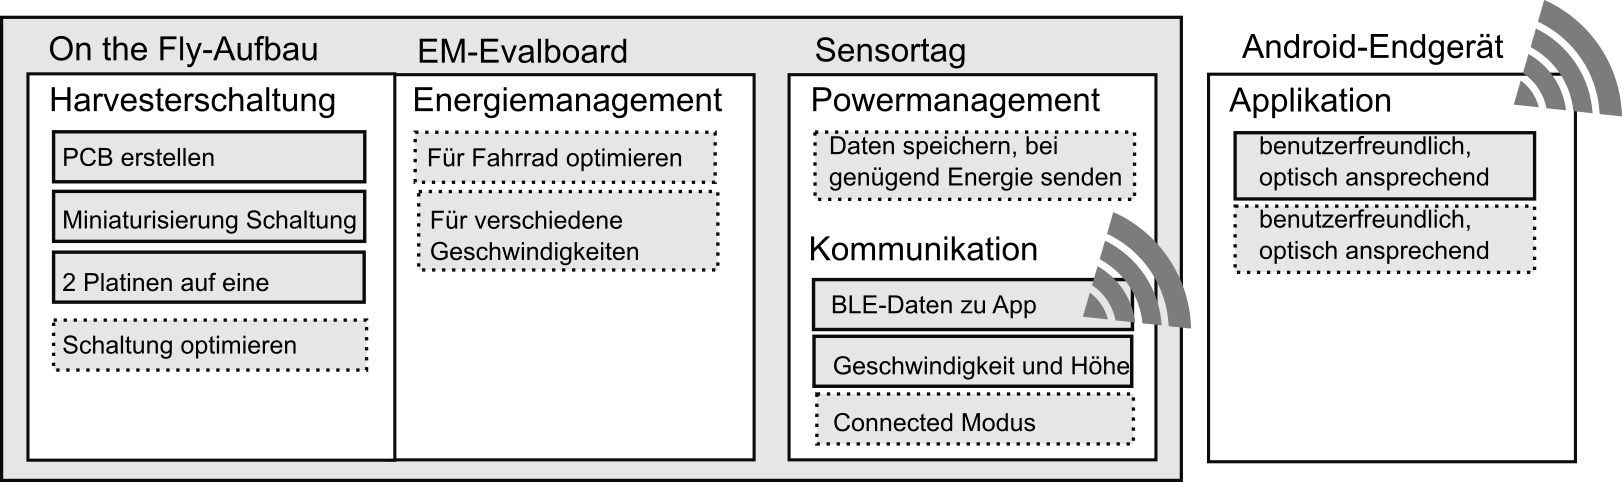
\includegraphics[width=1.0\textwidth]{../ressources/Projektorganisation/Arbeitsbloecke.png} 
    \caption{Arbeitsblöcke}
\end{figure}\label{arbeitsbloecke} 

